\documentclass[4paper,11pt]{report}
\author{Florian~Hirtz}


\usepackage[ngerman]{babel}
\usepackage[utf8]{inputenc}
\usepackage[export]{adjustbox}[2011/08/13]
\usepackage{minted}
\usepackage{caption}
\usepackage{blindtext}
\usepackage{graphicx}
\usepackage{fancyhdr}
\usepackage{subfiles}
\usepackage{hyperref}
\usepackage{pdfpages}

\newenvironment{code}{\captionsetup{type=figure}}{}
\newenvironment{image}{\captionsetup{type=figure}}{}

%minimale page header & footer
\pagestyle{fancy}
\setlength{\headheight}{14pt} 
\fancyhf{}
\fancyhead[C]{\nouppercase{\leftmark}}
\fancyfoot[C]{\thepage}

%Depth of sections
\setcounter{secnumdepth}{3}
\setcounter{tocdepth}{3}
\bibliographystyle{abbrv}

\graphicspath{./images/}

\title{Studnetz, eine Applikation für Mobilgeräte zur Vermittlung von Nachhilfeunterricht}

\begin{document}
	%\maketitle	
	\pagenumbering{gobble}
	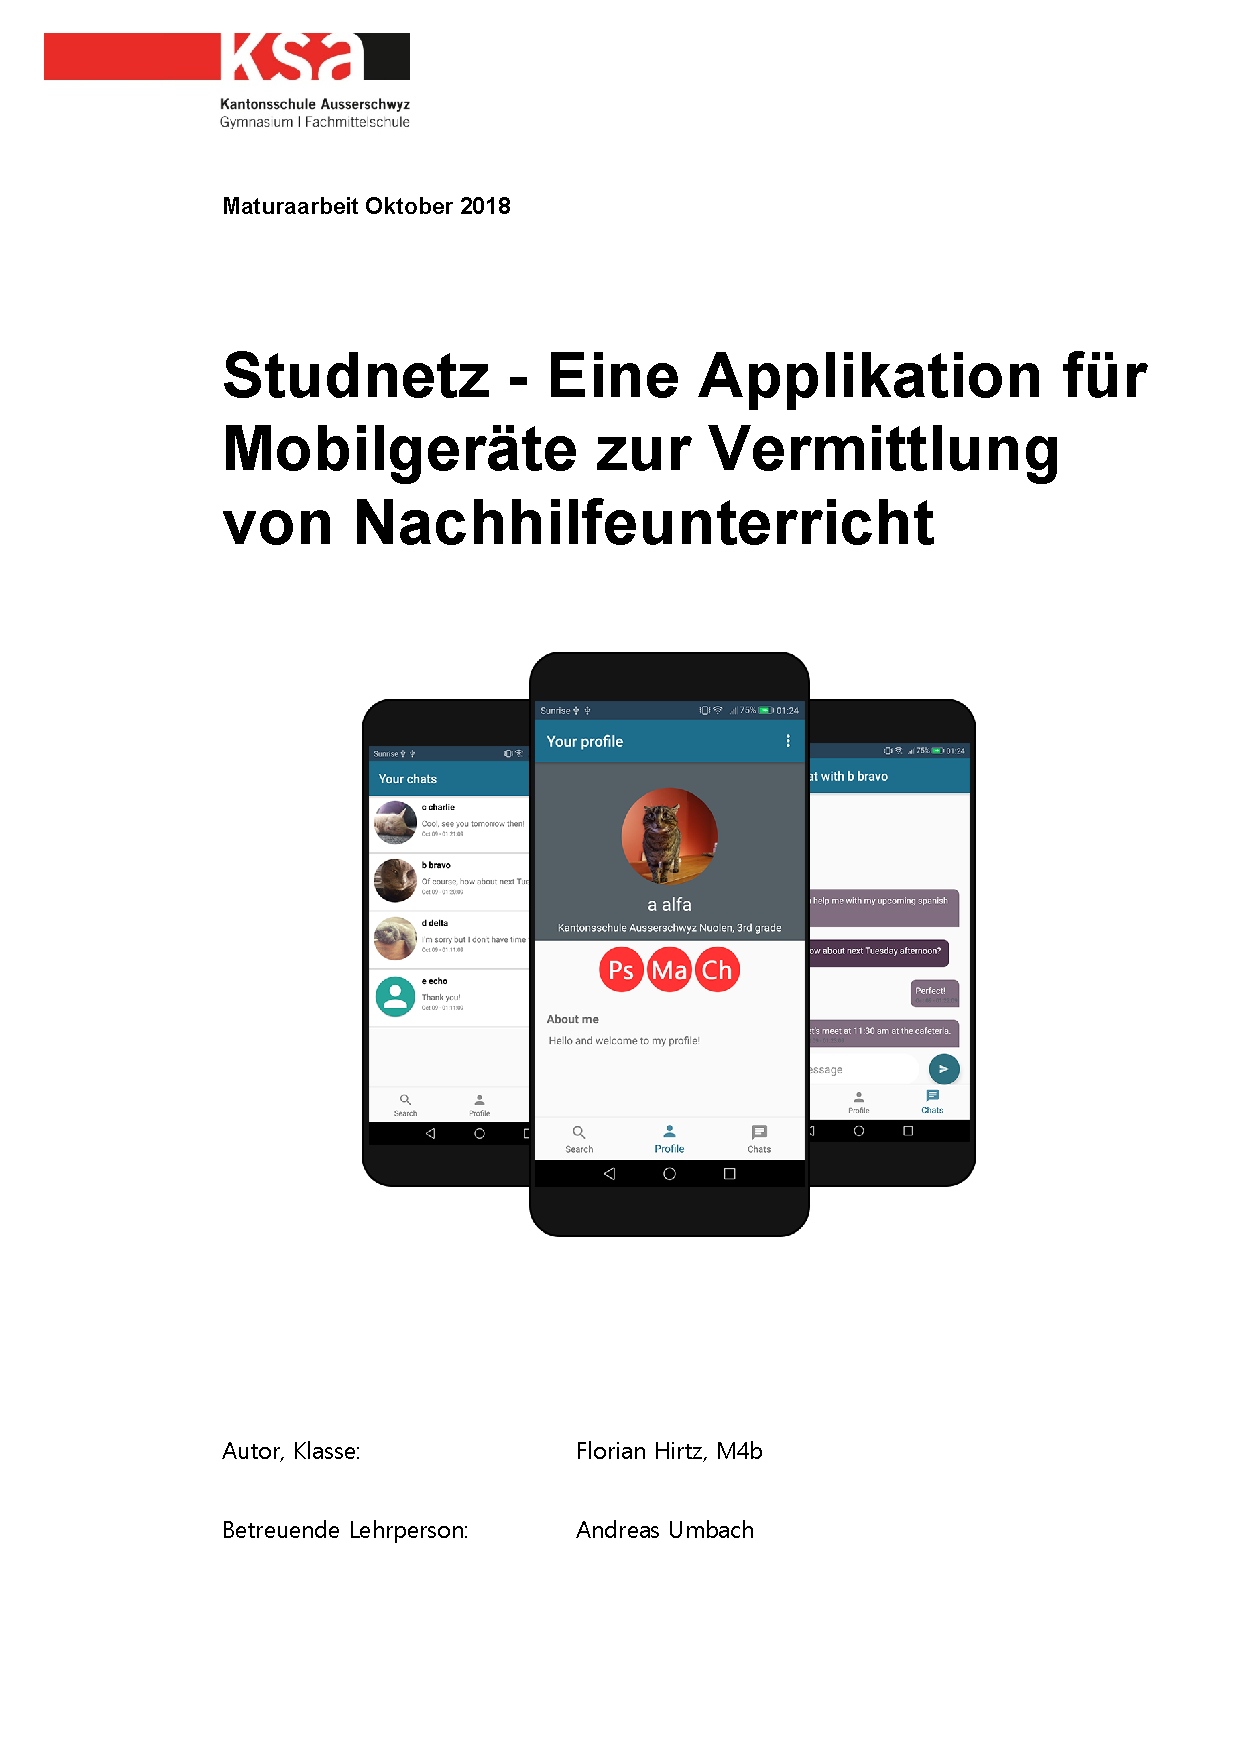
\includepdf[pages={1}]{titlepage.pdf}
	\pagenumbering{arabic}
	\tableofcontents
	
	\newpage
	\subfile{chapters/abstract.tex}
	\addcontentsline{toc}{chapter}{Abstract}
	\subfile{chapters/vorwort.tex}
	\addcontentsline{toc}{chapter}{Vorwort}
	%Corrected
	\subfile{chapters/Einleitung.tex}
	
	
	%Corrected
	\subfile{chapters/Konzeptionelle_Grundlagen.tex}
	%Rewriten, not yet Corrected
	\subfile{chapters/Die_entwickelte_Applikation}
	%Uncorrected
	%TODO: Schema von Client und Server für Studnetz
	\subfile{chapters/Die_Server}
	%Uncorrected
	\subfile{chapters/Der_Client}
	%Uncorrected
	
	\subfile{chapters/Arbeitsprozess.tex}
	
	\subfile{chapters/Diskussion}
	
	{\raggedright
		\listoffigures
		\bibliography{literatur}
	}

	\newpage
	
	
	
	
\end{document}